\documentclass{article}
\usepackage{fancyhdr}
\pagestyle{fancy}
\fancyfoot{}
\fancyfoot[C]{\thepage}
\rhead{Yarosevich - 1064712}
\usepackage{setspace}
\usepackage{siunitx} % Provides the \SI{}{} and \si{} command for typesetting SI units
\usepackage{graphicx} % Required for the inclusion of images
\usepackage{amsmath} % Required for some math elements 
\usepackage[export]{adjustbox} % loads also graphicx
\usepackage{listings}
\usepackage{setspace}
\usepackage{matlab-prettifier}
\usepackage{float}
\usepackage[many]{tcolorbox}
\usepackage[letterpaper, margin=1.2in]{geometry}
\usepackage{xcolor}
\usepackage{amsfonts}
\usepackage{color}
\usepackage{physics}
\usepackage{titlesec}
\usepackage{caption}
\usepackage{subcaption}
\usepackage{python}
\usepackage{placeins}
\usepackage{bm}
\usepackage{esvect}
\usepackage{mathtools}
\newcommand\Cb{\mathds{C}}
\newcommand\Eb{\mathds{E}}
\newcommand\Fb{\mathds{F}}
\newcommand\Gb{\mathds{G}}
\newcommand\Ib{\mathds{I}}
\newcommand\Pb{\mathds{P}}
\newcommand\Qb{\mathds{Q}}
\newcommand\Rb{\mathds{R}}
%\newcommand\Zb{\mathds{Z}}
\newcommand\Nb{\mathds{N}}
\newcommand\Vb{\mathds{V}}
\newcommand\Ub{\mathds{U}}
\usepackage{amssymb}  % gives you \mathbb{} font
\usepackage{dsfont}	% gives you \mathds{} font
\newcommand{\uveci}{{\bm{\hat{\textnormal{\bfseries\i}}}}}
\newcommand{\uvecj}{{\bm{\hat{\textnormal{\bfseries\j}}}}}
\DeclareRobustCommand{\uvec}[1]{{%
  \ifcsname uvec#1\endcsname
     \csname uvec#1\endcsname
   \else
    \bm{\hat{\mathbf{#1}}}%
   \fi
}}
\lstset{
  basicstyle=\ttfamily,
  columns=fullflexible,
  frame=single,
  breaklines=true,
  postbreak=\mbox{\textcolor{red}{$\hookrightarrow$}\space},
}


\newcommand{\R}{\mathbb{R}}

\usepackage{xcolor}

\DeclareCaptionFont{white}{\color{white}}
\DeclareCaptionFormat{listing}{%
  \parbox{\textwidth}{\colorbox{gray}{\parbox{\textwidth}{#1#2#3}}\vskip-4pt}}
\captionsetup[lstlisting]{format=listing,labelfont=white,textfont=white}
\lstset{frame=lrb,xleftmargin=\fboxsep,xrightmargin=-\fboxsep}
\titleformat{\section}[runin]
  {\normalfont\Large\bfseries}{\thesection}{1em}{}
\titleformat{\subsection}[runin]
  {\normalfont\large\bfseries}{\thesubsection}{1em}{}


\setlength\parindent{0pt} % Removes all indentation from paragraphs

\renewcommand{\labelenumi}{\alph{enumi}.} % Make numbering in the enumerate environment by letter rather than number (e.g. section 6)

%\usepackage{times} % Uncomment to use the Times New Roman font

%----------------------------------------------------------------------------------------
%	DOCUMENT INFORMATION
%----------------------------------------------------------------------------------------

\title{AMATH 522: Homework 3 \\Due November, 20 2019 \\ ID: 1064712} % Title

\author{Trent \textsc{Yarosevich}} % Author name

\date{\today} % Date for the report

\begin{document}
\maketitle % Insert the title, author and date
\setlength\parindent{1cm}

\begin{center}
\begin{tabular}{l r}
%Date Performed: December 1, 2017 \\ % Date the experiment was performed
Instructor: Professor Eric Shea-Brown % Instructor/supervisor
\end{tabular}
\end{center}
\doublespacing
% If you wish to include an abstract, uncomment the lines below
% \begin{abstract}
% Abstract text
% \end{abstract}

%----------------------------------------------------------------------------------------
%	SECTION 1
%----------------------------------------------------------------------------------------
\section*{\textbf{(Problem 1 - Coupled Oscillators)}}
This exercise is mostly comprised of code, so I have that listed below and I've tried to comment it clearly. We are also asked to address the following questions:
\begin{tcolorbox}[minipage,colback=gray!30!white,title = \large{\textbf{(i)}}, arc=0pt,outer arc=0pt]
Do nonzero values of $\gamma$ serve to synchronize the two oscillators? Does it matter whether $\gamma$ is positive or negative? Give some intuition for the effects of $\gamma$.
\end{tcolorbox}
To answer the first and third questions, the repressing proteins are coupled to each other with strength $\gamma$ and they repress their respective proteins. Now, the mRNA that these repressing factors each affect are not directly coupled, however their repressing factors are. This is to say, when $m_1$'s repressing factor $p_1$ is high, it represses $m_1$ with more strength, \textbf{and} it is coupled to $q_1$ in a positive way, so it also increases $q_1$'s production which allows it to suppress $n_1$ even more. An inverse relationship also holds. As a result, $n_1$ and $m_1$ converge with positive $\gamma$, along with $p_1$ and $q_1$. Similar logic holds for each other pairing.\\
\\
If $\gamma$ is negative, physically incoherent things happen, since any repressing protein that starts higher than the one it is coupled to will blow up, and the one it is coupled to will crash to negative values. As a result, mRNA with negative repressing proteins blow up, and ones with positive repressing proteins eventually reach zero.\\
\\
What's strange is what we get with very small negative $\gamma$, namely complex oscillations - indeed they appear to me to have some kind of period doubling (illustrated in the last plot), which suggests that some chaotic phenomena is at play. This seems highly plausible since we are dealing with an oscillating mapping of six variables, and some terms that resemble the logistic map. As $-\gamma$ approaches some threshhold around $-.25$ we can clearly see a period-doubling route to chaotic behavior. Without diving into a very complicated analysis, I would specualate that the dynamics are being dominated by something resembling a logistic map. In any case I've included 4 plots showing the movement toward this period doubling route to chaos as it's pretty damn cool!\\
\\
The following three plots illustrate: (i) first wild oscillations; (ii) second, a very short time slice so we can clearly see there is no convergence; (iii) a relatively low $\gamma$ that illustrate the pairwise convergence; (iv) the hint of chaotic behavior with $\gamma = -.1, -.2, -.235, -.27$.
\begin{center}
    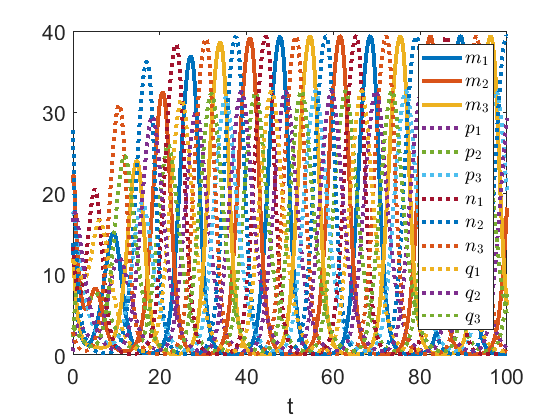
\includegraphics[scale = .8]{part_1_oscillations.png}
    \captionof{figure}{$\alpha = 50,\text{ } \beta =.5,\text{ } n=2, \text{ } \gamma = 0$}
    %\label{fig: D}
\end{center}
\begin{center}
    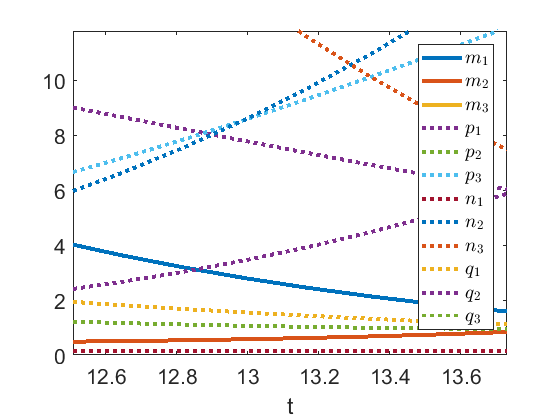
\includegraphics[scale = .8]{part_1_closeup.png}
    \captionof{figure}{$\alpha = 50,\text{ } \beta =5,\text{ } n=2, \text{ } \gamma = 0$}
    %\label{fig: D}
\end{center}


\begin{center}
    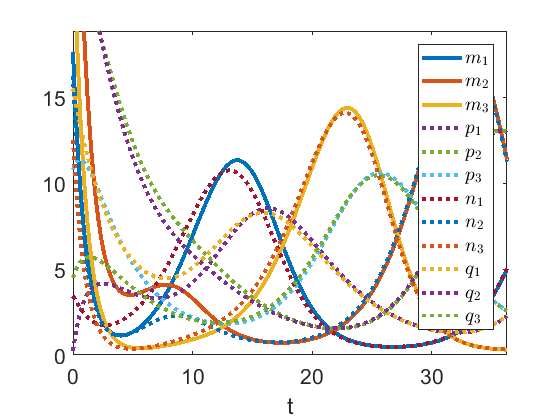
\includegraphics[scale = .8]{part1_1_fig.png}
    \captionof{figure}{$\alpha = 50,\text{ } \beta =.2,\text{ } n=2, \text{ } \gamma = .1$}
    %\label{fig: D}
\end{center}
several periods = -.1   lots of periods= -.2 over a longer timespan (1000)
 weirdness = -.235  
\begin{center}
    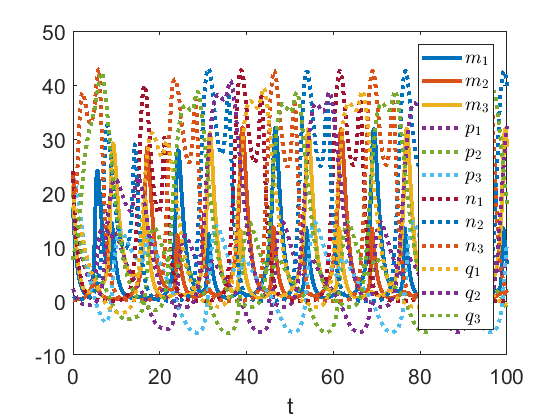
\includegraphics[scale = .5]{several_periods.png}
    %\captionof{figure}{$\gamma = -.1$}
    %\label{fig: D}
        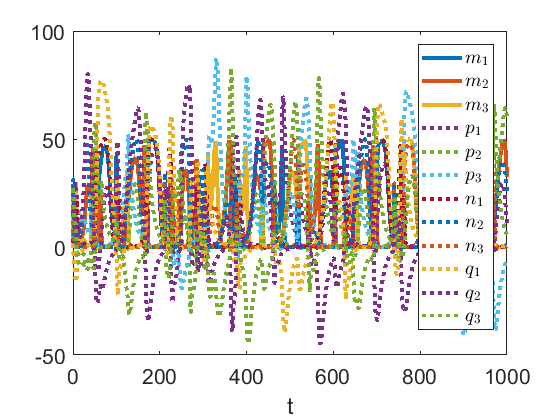
\includegraphics[scale = .5]{lots_of_periods.png}
    %\captionof{figure}{$\gamma = -.2$}
    %\label{fig: D}
        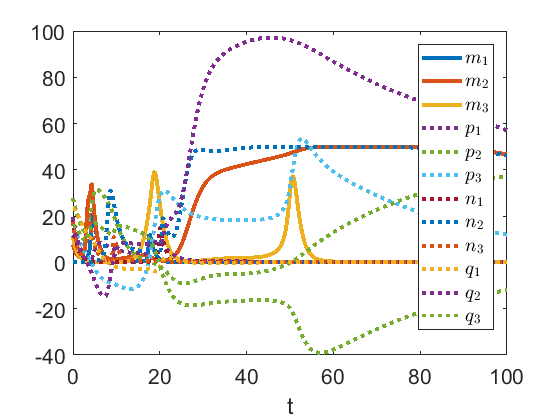
\includegraphics[scale = .5]{weirdness.png}
    %\captionof{figure}{$\gamma = -.235$}
    %\label{fig: D}
        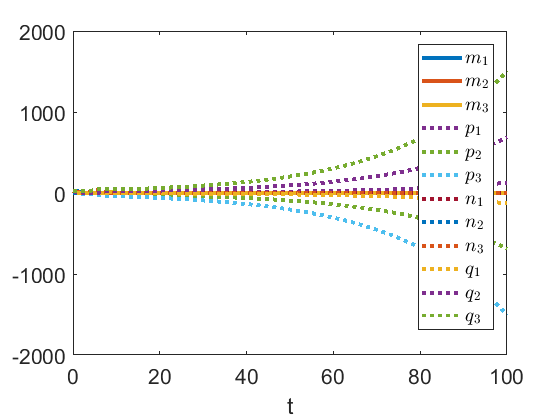
\includegraphics[scale = .5]{crash.png}
    %\captionof{figure}{$\gamma = -.27$}
    %\label{fig: D}
\end{center}
\section*{\textbf{(Problem 2 - Replicating Figures)}}
\subsection*{\textbf{(7.a)}}

 I structured my dynamics very literally from the motif schematic, namely using an overall growth function taken from the class notes for an activator: $\frac{\beta x^n}{K^n + x^n}$. I then assumed decay of rate $-\gamma x$. I then assumed, since $Y$ and $Z$ are activating $X$, and $X$ and $Z$ are activating $Y$ I wrote these activation equations accordingly (though I left the decay terms for $X$ in terms of $X$ etc). Then using the insight from Alson's paper, that the dynamics were of the form $\frac{dX}{dt} = F(Y,Z) - aX$ I simply included $Z$ as a constant influx beginning at $t=2$ and ending at $t=4$. Thus in essence, $Z$ 'bumps' $X$ and $Y$ into activation, and they continue after it is gone with 'memory':
\begin{equation}
\begin{aligned}
\frac{dX}{dt} = \frac{\alpha (Y+Z)^n}{1 + (Y+Z)^n} - aX\\
\frac{dY}{dt} = \frac{\alpha (X+Z)^n}{1 + (X+Z)^n} - aY\\
\end{aligned}
\end{equation}
These dynamics gave me the following figures:
\begin{center}
    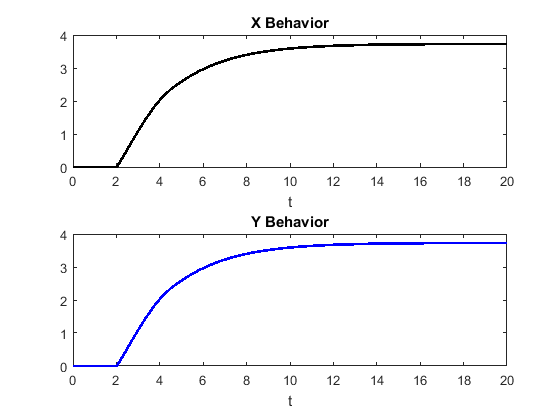
\includegraphics[scale = 1]{7a.png}
    %\captionof{figure}{D}
    %\label{fig: D}
\end{center}
Here is the RHS update:
\begin{lstlisting}[language=Matlab]
function dy = posfeed(t,y,p)
    if (2<t) && (t<4)
        z = 1;
    else
        z = 0;
    end
    dy = zeros(2,1);
    dy(1) = ( p(1)*(y(2) + z)^p(4)) / (1 + (y(2) + z)^p(4)) - p(3)*y(1); 
    dy(2) = ( p(2)*(y(1) + z)^p(4)) / (1 + (y(1) + z)^p(4)) - p(3)*y(2);
\end{lstlisting}
And the script:
\begin{lstlisting}[language=Matlab]
% Simulate the repressilator model
% Positive Feedforward loop

alpha=2;
beta =2;
gamma = .5;
n = 2;
k=1;

p = [alpha, beta, gamma, n, k];
y0 = [0, 0];
tmax = 20;

[T,Y] = ode45(@posfeed,[0, tmax],y0,[],p);



subplot(2,1,1);
plot(T,Y(:,1), 'k', 'LineWidth', 2)
title('X Behavior')
xlabel('t')
subplot(2,1,2);
plot(T,Y(:,2), 'b',  'LineWidth', 2)
xlabel('t')
title('Y Behavior')
\end{lstlisting}
\subsection*{\textbf{(7b)}}

For this one, by the time I had moved on and worked through \textbf{(7.c.)} I felt I started to understand the problems, and I realized I had not done this one correctly. I have qualitatively replicated the dynamics, but the resemblance of the dynamics to the motif are not good. I used the following:
\begin{equation}
\begin{aligned}
\frac{dX}{dt} = \frac{\alpha(Z + X)^2}{1+(X+Z)^2}(\frac{\alpha}{1+Y^2}) - \gamma X\\
\frac{dY}{dt} = -(X+Z)(\frac{\alpha Y}{1+(X+Z)^2})
\end{aligned}
\end{equation}
I think my intention was to write Y's dynamics like a repressing protein multiplied by a repressing term from $X$ and $Z$, and $X$ as an activating term in terms of $X$ and $Z$ with a repressing term from $Y$, but this isn't quite right. I'm not sure why the dynamics worked out, but they did:
\begin{center}
    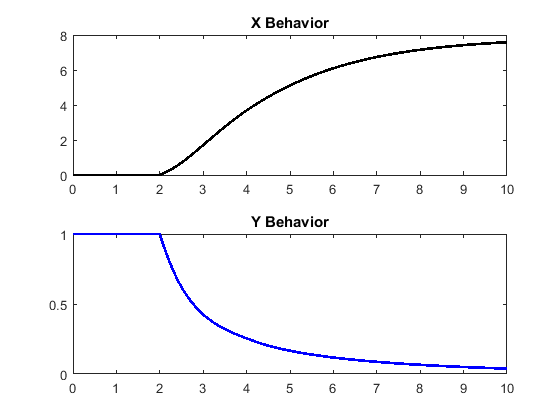
\includegraphics[scale = 1]{7b.png}
    %\captionof{figure}{D}
    %\label{fig: D}
\end{center}
Again the RHS update:
\begin{lstlisting}[language=Matlab]
function dy = negfeed(t,y,p)
 
    if (2<t) && (t<4)
        z = 1;
    else
        z = 0;
    end
    dy = zeros(2,1);
    dy(1) = ( p(1) * (z + y(1))^p(4) ) /(1 + (y(1) + z)^p(4))*(p(1) / (1+y(2)^2)) - p(3)*y(1); 
    dy(2) = - (y(1) + z)* (y(2))*(p(1) / (1+(z +y(1))^2));

\end{lstlisting}
And the script:
\begin{lstlisting}[language=Matlab]
clc; clear all; close all;

alpha=2;
beta =2;
gamma = .5;
n = 2;
k=1;

p = [alpha, beta, gamma, n, k];
y0 = [0, 1];
tmax = 10;

[T,Y] = ode45(@negfeed,[0, tmax],y0,[],p);



subplot(2,1,1);
plot(T,Y(:,1), 'k', 'LineWidth', 2)
title('X Behavior')
subplot(2,1,2);
plot(T,Y(:,2), 'b',  'LineWidth', 2)
title('Y Behavior')
\end{lstlisting}
\subsection*{\textbf{(7.c)}}
This one is pretty complicated, so I tried to comment the code below to illustrate. I basically used the motifs very literally, structuring the dynamics as stated in the motifs where $Y_1$ is a repressing protein that also jointly activates $X_2$, etc. I used dynamics taken from the repressilator model. I also used master threshhold equations for $X_1$ and $X_2$, as Alson, 2002 does, but I only used the threshold as a delay - the effect once the threshhold is reached is constant, so it really just acts as a delayed on-off switch. This felt a little 'hacky' but intuitively I think it makes sense, since it could just be some binding saturation being reached that then activates a process with memory.\\
\\
The only wonky thing I had to do was to tweak the repressing terms to have threshholds very close to zero so that $Z_1$ and $Z_2$ would crash all the way down to zero, as opposed to crashing close to it. Setting the threshhold AT zero obviously produced division by zero errors. Below is the figure I produced, and carefully commented code.
\begin{center}
    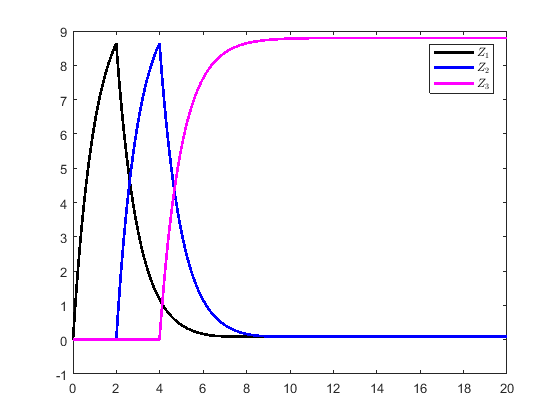
\includegraphics[scale = 1]{7c.png}
    %\captionof{figure}{D}
    %\label{fig: D}
\end{center}
Here is the RHS update function:
\begin{lstlisting}[language=Matlab]
function dy = sharktooth(t,y,p)
    % Condition on the threshhold equation that immediately starts 
    % production of Z1.
    if y(1) > 0
        z1=1;
    else
        z1=0;
    end
    % Condition on threshhold equation to start production of Y1 
    % a little later.
    if y(1) > 1.5
        z2 = 1;
    else
        z2=0;
    end
    % If condition to start X2 as soon as X1 and Y1 are being made.
    % Represents saturation by an activating protein.
    if y(3) > 0
        z3 = 1;
    else 
        z3=0;
    end
    % Threshhold condition for delayed production of Y2.
    if y(4) > 1.5
        z4 = 1;
    else
        z4=0;
    end
    dy = zeros(7,1);
    % Threshhold dynamics to represent X1 activating 
    % Z1 and then afterward Y1.
    dy(1) = 1 - .3*y(1);
    
    % Corresponds to Z1. Activation is assumed to be immediate by X1, along
    % with a repression term from Y1.
    dy(2) = p(1) / (.0001 + y(3)^2) - y(2);
    
    % Corresponds to Y1, a repressing protein.
    dy(3) = -z2*p(2) * (y(3) - y(2)) ;
    
    % Threshhold equation to represent X2 for delayed activation of Z2 and
    % Y2.
    dy(4) = z3 - .3*y(4);
    
    % Corresponds to Z2, analogous to Z2 above.
    dy(5) = z3*p(1) / (.0001 + y(6)^2) - y(5);
    
    % Corresponds to Y2, analogous to Y2 above.
    dy(6) = -z4*p(2) * (y(6) - y(5));
    
    % Corresponds to Z3, which is just a growth equation with decay.
    dy(7) = 8.8*z4 - y(7);
\end{lstlisting}
And here is the script:
\begin{lstlisting}[language=Matlab]
clc; clear all; close all;

alpha=.001;
beta = 5;
gamma =1;
n = 1;
k=1;

p = [alpha, beta, gamma, n, k];
y0 = [0, 0, 0, 0, 0, 0, 0];
tmax = 20;

[T,Y] = ode45(@sharktooth,[0, tmax],y0,[],p);

figure(1)
plot(T,Y(:,2), 'k', 'LineWidth', 2)
title('')
hold on;
plot(T, Y(:,5), 'b', 'LineWidth', 2)
plot(T, Y(:,7), 'm', 'LineWidth', 2)
legend({'$Z_1$', '$Z_2$', '$Z_3$'}, 'Interpreter', 'latex')
\end{lstlisting}
 \end{document}
